\documentclass[10pt, nofootinbib, twocolumn]{revtex4-1}
\usepackage{amsmath}
\usepackage{xparse}
\usepackage{graphicx}
\usepackage{hyperref}
\usepackage{color}
\usepackage{physics}
\usepackage{enumitem}
\usepackage{natbib}
\usepackage{booktabs}
\usepackage{float}
\usepackage{caption}
\usepackage{mathtools}
\usepackage{multirow}

\hypersetup{
    colorlinks=true,
    linkcolor=black,  
    citecolor=black,
    urlcolor=blue
}


\begin{document}

\title{Project3 AST3310 - Stellar Convection} 
\date{\today} \homepage{https://github.com/tirilsg/AST3310_Project3}       
\begin{abstract}
    \textit{A model of the convective zone at the surface of a star equating the photosphere of the sun is developed by in this report. This model is used to run 2D simulations visualizing the behaviours of rising parcels of heated gas, with characteristics described by hydrodynamic equations.}
\end{abstract}
\maketitle       

\section{Introduction}\label{sec:introduction}
A star is fueled by thermally ignited nuclear fusion. The transportation of this energy is modelled by assuming only ideal gasses, and occurs mostly in the form of radiation - energy-retaining photons travelling through the body and escaping the surface of the star. Whenever the amount of energy produced exceeds the ability for transportation to occur solely by radiation, the excess energy heats up the gas allowing it to become unstable and raise toward the surface - convection becomes an active method of energy transportation. \\

Previously, we've simulated the energy transportation occurring in a star after the surface-defining variables radius r, density $\rho$, luminosity L, temperature T and mass m, depending on only the distance from the stellar centre, and thereby also in a single dimension. A continuous zone of convection was constructed at the stellar surface. In this project, we wish to create a more accurate simulation of this convection-zone in two dimensions. \\

In order to model the behaviour of the gas, we make use of the fluid description theory that is hydrodynamics. We construct a two-dimensional space, and apply the rules of hydrodynamics, and allow for systems with different initial temperature distributions to evolve in time. A sanity check is exerted, confirming the soundness of the model. Thereafter, the model is used to simulate the behaviour exerted whenever we initialize the system with both a single, and five distinct temperature disturbances. The behaviour observed subsequently is discussed, and a conclusion is drawn in light of this debate.




\section{Theory}\label{sec:theory}
The requirement for a medium to be qualified as a liquid, and thereby be described by the laws of hydrodynamics, is that \textit{it can be split into volume elements which can be represented by a continuous function $\rho$ defined by} \cite{ast}
\begin{equation}
    \rho dV = \sum_{dV}{m}
\end{equation}
where dV represents the volume element, and m is the mass of the particles making up the fluid; $\rho$ thereby denotes the mass density. This requirement is applicable to the convection zone, which allows for a behavioural description by hydrodynamics. Said behaviours are denoted by the Momentum Equation \eqref{eq:momentum}, Continuity Equation \eqref{eq:continuity} and Energy Equation \eqref{eq:energy}.

\subsection{The Momentum Equation}
The equation describing the momentum, takes into account the external body forces working on the fluid, in this case gravity, is given by Equation \eqref{eq:momentum} \cite{text}
\begin{equation}\label{eq:momentum}
    \frac{\partial \rho \vec{u}}{\partial t}+\nabla \cdot (\rho \vec{u}\otimes\vec{u})=-\nabla P +\rho \vec{g}
\end{equation}
where $\rho$ is the density of mass, P is the thermal pressure, $\vec{u}=u\vec{i}+w\vec{j}$ is the velocity vector, $\nabla$ is the differential operator, and $\vec{g}=g\vec{j}=\frac{GM}{r^2}$ is the gravitational acceleration in the y-direction, defined by the constant G, mass M = $M_\odot$ and radius R = $R_\odot$ defined in Table \ref{tab:const}, which we assume to only work in the y-direction in order to create a space resembling that of the photosphere of the sun. This equation takes into account gravity, but excludes the stress tensor \cite{ast}. The operator $\otimes$ denotes a tensor product, allowing for the Momentum Equation \eqref{eq:momentum} to be expanded, and subsequently rewritten in terms of x- and y-coordinates, which will become beneficial.
\begin{equation}
    \frac{\partial \rho u }{\partial t}\hat{i} + \frac{\partial \rho w }{\partial t}\hat{j} +(\frac{\partial \rho u }{\partial x} + \frac{\partial \rho w }{\partial y})(u\hat{i}+w\hat{j}) = - \frac{\partial P}{\partial x} -\frac{\partial P}{\partial y} + \rho g \hat{j}
\end{equation}
\begin{equation}\label{eq:mom_u}
\begin{split}
     \frac{\partial \rho u }{\partial t} = -\frac{\partial \rho u^2}{\partial x}-\frac{\partial \rho uw}{\partial y}-\frac{\partial P}{\partial x} \\
     = -\rho u \left( \frac{\partial u}{\partial x} +\frac{\partial w}{\partial y} \right) -u\frac{\partial \rho u}{\partial x}-w\frac{\partial \rho u}{\partial y}-\frac{\partial P}{\partial x} \\
\end{split}
\end{equation}
\begin{equation}\label{eq:mom_w}
\begin{split}
    \frac{\partial \rho w }{\partial t} = -\frac{\partial \rho w^2}{\partial y}-\frac{\partial \rho uw}{\partial x}-\frac{\partial P}{\partial y}+\rho g \\
    = -\rho w \left( \frac{\partial u}{\partial x} +\frac{\partial w}{\partial y} \right)-u\frac{\partial \rho w}{\partial x}-w\frac{\partial \rho w}{\partial y}-\frac{\partial P}{\partial y}+\rho g 
\end{split}
\end{equation}


\subsection{The Continuity Equation}
The Continuity Equation \eqref{eq:continuity} describes how the behaviours occurring within the system might affect the distribution of mass, the density $\rho$. 
\begin{equation}\label{eq:continuity}
    \frac{\partial \rho}{\partial t}+\nabla \cdot (\rho \vec{u})=0
\end{equation}
Equation \eqref{eq:continuity} does not take into consideration source or sink terms, and is therefore also describing a conservation of mass within the system. The Equation \eqref{eq:continuity} can be rewritten to Equation \eqref{eq:cont_exp}
\begin{equation}\label{eq:cont_exp}
\begin{split}
    \frac{\partial \rho}{\partial t}=-\frac{\partial \rho u}{\partial x} -\frac{\partial \rho w}{\partial y} \\
     = -\rho\left( \frac{\partial u}{\partial x} +\frac{\partial w}{\partial y} \right)-u\frac{\partial \rho }{\partial x}-w\frac{\partial \rho }{\partial y} \\
\end{split}
\end{equation}


\subsection{The Energy Equation}
In hydrodynamics, the description of internal energy e is used instead of the previously utilized temperature gradient. The behaviour of this internal energy is described by the Energy Equation \eqref{eq:energy} \cite {ast}
\begin{equation}\label{eq:energy}
    \frac{\partial e}{\partial t}+\nabla \cdot (e \vec{u})=-P\nabla \cdot \vec{u}
\end{equation}
where e is the internal energy per unit mass, which we can define from the the equation of state for an ideal gas, Equation \eqref{eq:eqostate}
\begin{equation}\label{eq:eqostate}
    P=\frac{k_BT\rho}{\mu m_u}
\end{equation}
giving Equation \eqref{eq:internal_e}
\begin{equation}\label{eq:internal_e}
    e=\frac{P}{(\gamma-1)}=\frac{k_BT\rho}{\mu m_u(\gamma -1)}
\end{equation}
Here, $\gamma = c_P / c_V$ is the ratio of specific heats, which is constant for the gas we assume to be ideal, $\gamma = 5/3$ \cite[p.~58]{ast}.
The Equation \eqref{eq:energy} can be rewritten to express the change in energy as a function of time as in Equation \eqref{eq:en_exp}
\begin{equation}\label{eq:en_exp}
    \frac{\partial e}{\partial t}=-\left( u\frac{\partial e}{\partial x} +w\frac{\partial e}{\partial y} \right)- P \left( \frac{\partial u}{\partial x} +\frac{\partial w}{\partial y} \right)
\end{equation}


\section{Methods}\label{sec:methods} 
\subsection{Model}
The model is implemented by first defining a space xy-space, and dividing said volume into identical cubic cells, which can be viewed as pixels with dimensions $\Delta x$ and $\Delta y$ in the respective directions. Thereby, the volume will be divided into a total grid of size $\quad N_x  \Delta x \quad \times \quad N_y \Delta y \quad $ where N denotes the amounts of pixels making up the total volume. This allows us to describe the xy-space by discrete coordinates $$x_i = x_0 +i\Delta x \quad y_j = y_0 +j\Delta y \quad t_n = t_0 +n\Delta t$$ where we use i, j and n to navigate the xy- and t-space. 

\subsection{Discretization}
In order to be able to apply the equations describing how density, momentum and energy behaves as time passes to the model, the expressions for behaviours within the plasma need to be discretizised in the different directions x and y. This, we do by rewriting the Momentum Equations \eqref{eq:mom_u} and \eqref{eq:mom_w}, the Continuity Equation \eqref{eq:cont_exp} and the Energy Equation \eqref{eq:en_exp} . 
\begin{equation}\label{eq:cont_dis}
\begin{split}
       \left[\frac{\partial \rho}{\partial t}\right]^{n}_{i,j} =
    -\rho_{i,j}^n\left( \left[\frac{\partial u}{\partial x}\right]^{n}_{i,j} +  \left[\frac{\partial w}{\partial y}\right]^{n}_{i,j}  \right) \\
    -u_{i,j}^n\left[\frac{\partial \rho}{\partial x}\right]^{n}_{i,j}
    -w_{i,j}^n\left[\frac{\partial \rho}{\partial y}\right]^{n}_{i,j} 
\end{split}
\end{equation}
\begin{equation}\label{eq:momu_dis}
\begin{split}
        \left[\frac{\partial \rho u}{\partial t}\right]^{n}_{i,j} = 
    -[\rho u]_{i,j}^n\left( \left[\frac{\partial u}{\partial x}\right]^{n}_{i,j} +  \left[\frac{\partial w}{\partial y}\right]^{n}_{i,j}  \right) \\
    -u_{i,j}^n\left[\frac{\partial \rho u}{\partial x}\right]^{n}_{i,j}
    -w_{i,j}^n\left[\frac{\partial \rho u}{\partial y}\right]^{n}_{i,j}
    -\left[\frac{\partial P}{\partial x}\right]^{n}_{i,j}
\end{split}
\end{equation}
\begin{equation}\label{eq:momw_dis}
\begin{split}
    \left[\frac{\partial \rho w}{\partial t}\right]^{n}_{i,j} = 
    -[\rho w]_{i,j}^n\left( \left[\frac{\partial u}{\partial x}\right]^{n}_{i,j} +  \left[\frac{\partial w}{\partial y}\right]^{n}_{i,j}  \right) \\
    -u_{i,j}^n\left[\frac{\partial \rho w}{\partial x}\right]^{n}_{i,j}
    -w_{i,j}^n\left[\frac{\partial \rho w}{\partial y}\right]^{n}_{i,j}
    -\left[\frac{\partial P}{\partial y}\right]^{n}_{i,j}-\rho_{i,j}^n g
\end{split}
\end{equation}
\begin{equation}\label{eq:en_dis}
\begin{split}
     \left[\frac{\partial e}{\partial t}\right]^{n}_{i,j} = 
     -u_{i,j}^n\left[\frac{\partial e}{\partial x}\right]^{n}_{i,j}
    -w_{i,j}^n\left[\frac{\partial e}{\partial y}\right]^{n}_{i,j}\\
    - P_{i,j}^n \left( \left[\frac{\partial u}{\partial x}\right]^{n}_{i,j} +  \left[\frac{\partial w}{\partial y}\right]^{n}_{i,j}  \right)
\end{split}
\end{equation}
The spatial derivatives utilized in the discretized Equations \eqref{eq:cont_dis}-\eqref{eq:en_dis} are largely dependent on which direction the gas flows in. The derivatives are simply defined by the change in each variable in the respective directions, and must be defined dependent on the direction of flow. If the direction of flow is the same for the neighboring points, the difference between these can be used in a method known as \textbf{central differencing} \cite{text} in order to determine expressions for the behaviour occurring. Otherwise, this expression must be derived from the difference between the following or the previous point, depending on the direction of flow; 
$ u_{i,j}^{n} < 0$, $ w_{i,j}^{n} < 0$ denoting flow in negative directions, and $u_{i,j}^{n} \geq 0$, $w_{i,j}^{n} \geq 0$ denoting flow in positive direction. 

\subsubsection{Continuity Equation}
$$\left[\frac{\partial u}{\partial x}\right]^{n}_{i,j} = \frac{u_{i+1,j}^{n}-u_{i-1,j}^{n}}{2\Delta x}$$
$$\left[\frac{\partial w}{\partial y}\right]^{n}_{i,j} = \frac{w_{i,j+1}^{n}-w_{i,j-1}^{n}}{2\Delta y}$$
\[\left[\frac{\partial \rho }{\partial x}\right]^{n}_{i,j} = 
\begin{cases}
\frac{\rho_{i,j}^{n}-\rho_{i-1,j}^{n}}{\Delta x} & \text{if } u_{i,j}^{n} \geq 0 \\
\frac{\rho_{i+1,j}^{n}-\rho_{i,j}^{n}}{\Delta x} & \text{if } u_{i,j}^{n} < 0
\end{cases}\]
\[\left[\frac{\partial \rho }{\partial y}\right]^{n}_{i,j} = 
\begin{cases}
\frac{\rho_{i,j}^{n}-\rho_{i,j-1}^{n}}{\Delta y} & \text{if } w_{i,j}^{n} \geq 0 \\
\frac{\rho_{i,j+1}^{n}-\rho_{i,j}^{n}}{\Delta y} & \text{if } w_{i,j}^{n} < 0
\end{cases}\]

\subsubsection{Momentum Equation}
The Momentum Equation is divided into two expressions, Equation \eqref{eq:mom_u} and Equation \eqref{eq:mom_w}, denoting the horizontal and vertical momentum, respectively. \textbf{The Horizontal momentum expressions:}
\[\left[\frac{\partial u}{\partial x}\right]^{n}_{i,j} = 
\begin{cases}
\frac{u_{i,j}^{n}-u_{i-1,j}^{n}}{\Delta x} & \text{if } u_{i,j}^{n} \geq 0 \\
\frac{u_{i+1,j}^{n}-u_{i,j}^{n}}{\Delta x} & \text{if } u_{i,j}^{n} < 0
\end{cases}\]
\[\left[\frac{\partial \rho u}{\partial x}\right]^{n}_{i,j} = 
\begin{cases}
\frac{[\rho u]_{i,j}^{n}-[\rho u]_{i-1,j}^{n}}{\Delta x} & \text{if } u_{i,j}^{n} \geq 0 \\
\frac{[\rho u]_{i+1,j}^{n}-[\rho u]_{i,j}^{n}}{\Delta x} & \text{if } u_{i,j}^{n} < 0
\end{cases}\]
\[\left[\frac{\partial \rho u}{\partial y}\right]^{n}_{i,j} = 
\begin{cases}
\frac{[\rho u]_{i,j}^{n}-[\rho u]_{i,j-1}^{n}}{\Delta y} & \text{if } w_{i,j}^{n} \geq 0 \\
\frac{[\rho u]_{i,j+1}^{n}-[\rho u]_{i,j}^{n}}{\Delta y} & \text{if } w_{i,j}^{n} < 0
\end{cases}\]
$$\left[\frac{\partial P}{\partial x}\right]^{n}_{i,j} = \frac{P_{i+1,j}^{n}-P_{i-1,j}^{n}}{2\Delta x}$$
\textbf{The vertical momentum expressions:}
\[\left[\frac{\partial w}{\partial y}\right]^{n}_{i,j} = 
\begin{cases}
\frac{w_{i,j}^{n}-w_{i,j-1}^{n}}{\Delta y} & \text{if } w_{i,j}^{n} \geq 0 \\
\frac{w_{i,j+1}^{n}-w_{i,j}^{n}}{\Delta y} & \text{if } w_{i,j}^{n} < 0
\end{cases}\]
\[\left[\frac{\partial \rho w}{\partial x}\right]^{n}_{i,j} = 
\begin{cases}
\frac{[\rho w]_{i,j}^{n}-[\rho w]_{i-1,j}^{n}}{\Delta x} & \text{if } u_{i,j}^{n} \geq 0 \\
\frac{[\rho w]_{i+1,j}^{n}-[\rho w]_{i,j}^{n}}{\Delta x} & \text{if } u_{i,j}^{n} < 0
\end{cases}\]
\[\left[\frac{\partial \rho w}{\partial y}\right]^{n}_{i,j} = 
\begin{cases}
\frac{[\rho w]_{i,j}^{n}-[\rho w]_{i,j-1}^{n}}{\Delta y} & \text{if } w_{i,j}^{n} \geq 0 \\
\frac{[\rho w]_{i,j+1}^{n}-[\rho w]_{i,j}^{n}}{\Delta y} & \text{if } w_{i,j}^{n} < 0
\end{cases}\]
$$\left[\frac{\partial P}{\partial y}\right]^{n}_{i,j} = \frac{P_{i,j+1}^{n}-P_{i,j-1}^{n}}{2\Delta y}$$


\subsubsection{Energy Equation}
\[\left[\frac{\partial e}{\partial x}\right]^{n}_{i,j} = 
\begin{cases}
\frac{e_{i,j}^{n}-e_{i-1,j}^{n}}{\Delta x} & \text{if } u_{i,j}^{n} \geq 0 \\
\frac{e_{i+1,j}^{n}-e_{i,j}^{n}}{\Delta x} & \text{if } u_{i,j}^{n} < 0
\end{cases}\]
\[\left[\frac{\partial e}{\partial y}\right]^{n}_{i,j} = 
\begin{cases}
\frac{e_{i,j}^{n}-e_{i,j-1}^{n}}{\Delta y} & \text{if } w_{i,j}^{n} \geq 0 \\
\frac{e_{i,j+1}^{n}-e_{i,j}^{n}}{\Delta y} & \text{if } w_{i,j}^{n} < 0
\end{cases}\]



\subsection{Initial Conditions}
The initial condition of the system is defined by the two following requirements. The first requirement states that the gas needs to be in hydrostatic equilibrium. This means the forces of gravity are balanced by a pressure gradient force, keeping the equilibrium even though the distance from the mass-centre increases. \\

The second requirement is that the double logarithmic gradient $\nabla$ be larger than 2/5 in order to ensure that convection occurs. This is following the definition of the adiabatic temperature gradient , which denotes total energy transportation due to radiation. These requirements allows us to calculate the temperature and pressure from the values on the top of the box, which we model after the photosphere of the sun - the layer where most of the suns energy is emitted \cite{solar} from the stellar body into its surroundings. The change in temperature is described by the Equation \eqref{eq:t_y}
\begin{equation}\label{eq:t_y}
\begin{split}
    \frac{\partial T}{\partial y} = \nabla \frac{T\partial P}{P\partial y} \Rightarrow \nabla = \frac{P}{T}\frac{\partial T}{\partial P}
\end{split}
\end{equation}
Since the system is in a hydrostatic equilibrium, the change in pressure is only due to the external force of gravity, and is thereby described by the Equation \eqref{eq:p_y}
\begin{equation}\label{eq:p_y}
    \frac{\partial P}{\partial y} = -\rho \vec{g}
\end{equation}
Taking both Equation \eqref{eq:t_y} and Equation \eqref{eq:p_y} into consideration, the following expressions can be derived
\begin{equation}\label{eq:t}
\begin{split}
    \frac{\partial T}{\partial y} = \nabla \frac{T\partial P}{P\partial y}= \nabla \frac{(-\rho \vec{g})\mu m_u}{k_B\rho} \\
    \Rightarrow (T-T_0) = -\nabla \frac{ \vec{g}\mu m_u}{k_B}(y-y_0)\\ T=T_0-\nabla \frac{ \vec{g}\mu m_u}{k_B}(y-y_0)
\end{split}
\end{equation}
where $T_0=T_\odot$ denotes the temperature at the surface of the star.
\begin{equation}\label{eq:p}
\begin{split}
    \nabla = \frac{P}{T}\frac{\partial T}{\partial P} \Rightarrow \frac{\partial P}{P} =\frac{\partial T}{T}\nabla^{-1}\\ \int_{P_0}^P{\frac{\partial P}{P}}=\nabla^{-1}\int_{T_0}^T{\frac{\partial T}{T}}\\ ln\left(\frac{P}{P_0}\right)=\nabla^{-1}ln\left(\frac{T}{T_0}\right)\\ \Rightarrow P = P_0\left(\frac{T}{T_0}\right)^{\nabla^{-1}}
\end{split}
\end{equation}
where $P_0=P_\odot$ denotes the pressure at the surface of the star.
Lastly, the initial condition for velocity needs to be zero everywhere. \\



\subsection{Evolution in Time}
\subsubsection{Time Step}
The system is simply evolved in time by deriving equations from the discretized expressions; \\
\begin{equation}\label{eq:rho_e}
    \rho_{i,j}^{n+1} = \rho_{i,j}^{n}+\left[\frac{\partial \rho }{\partial t}\right]^{n}_{i,j} \Delta t
\end{equation}
\begin{equation}\label{eq:u_e}
    u_{i,j}^{n+1} = \frac{[\rho u]_{i,j}^n+\left[\frac{\partial \rho u}{\partial t}\right]^{n}_{i,j}\Delta t}{\rho_{i,j}^{n+1}}
\end{equation}
\begin{equation}\label{eq:w_e}
    w_{i,j}^{n+1} = \frac{[\rho w]_{i,j}^n+\left[\frac{\partial \rho w}{\partial t}\right]^{n}_{i,j}\Delta t}{\rho_{i,j}^{n+1}}
\end{equation}
\begin{equation}\label{eq:e_e}
    e_{i,j}^{n+1} = e_{i,j}^{n} + \left[\frac{\partial e}{\partial t}\right]^{n}_{i,j} \Delta t
\end{equation}
Temperature and pressure can be evolved in time by making use of the definitions of pressure by Equation \eqref{eq:eqostate} and internal energy by Equation \eqref{eq:eqostate}
\begin{equation}
    P_{i,j}^{n+1}=e_{i,j}^{n+1}(\gamma-1)
\end{equation}
\begin{equation}
    T_{i,j}^{n+1}=\frac{P_{i,j}^{n+1}}{\rho_{i,j}^{n+1}}\frac{\mu m_u}{k_B}
\end{equation}

\subsubsection{Time Step Size}
The size of the step in time $\Delta t$ is determined by first determining the largest relative change of all relevant variables u,w,e and $\rho$ per time step length $\delta$, and subsequently defining the time step by Equation \eqref{eq:dt}
\begin{equation}\label{eq:dt}
    \Delta t = \frac{p}{\delta}
\end{equation}
where p is a constant used to scale the step size as needed, commonly set to 0.1. $\delta$ is simply defined by the Equation \eqref{eq:delta}
\begin{equation}\label{eq:delta}
    \delta = max(max(\abs{\frac{\partial \phi}{\partial t}\cdot\frac{1}{\phi}}))
\end{equation}
where $\phi$ is replaced by  each primary variable, in order to finally retrieve the expression for $\delta$. 


\subsection{Boundary Conditions}
Lastly, the boundaries of the volume needs to be defined. \textbf{The boundaries for x} is defined as periodic, meaning
$$\phi_{-1,j}^n=\phi_{N_x-1,j}^n \qquad \vee \qquad \phi_{N_x,j}^n=\phi_{0,j}^n$$
which are boundaries applicable to all primary variables. \textbf{The boundaries on the y-axis} varies with the variables in question. The vertical boundary for vertical velocity is zero at the boundaries
$$w^{n}_{i,0}=w^{n}_{i,N_y-1}=0$$
The vertical boundary to the horizontal velocity, on the other hand, needs to be derived from either the three-point \textbf{forward difference approximation} \cite{text} given by Equation \eqref{eq:for}
\begin{equation}\label{eq:for}
    \left[\frac{\partial \phi}{\partial y}\right]^{n}_{i,j} = \frac{-\phi_{i,j+2}^n+4\phi_{i,j+1}^n-3\phi_{i,j}^n}{2\Delta y}
\end{equation}
or the three-point \textbf{backward difference approximation} \cite{text} given by Equation \eqref{eq:back}
\begin{equation}\label{eq:back}
    \left[\frac{\partial \phi}{\partial y}\right]^{n}_{i,j} = \frac{3\phi_{i,j}^n-4\phi_{i,j-1}^n+\phi_{i,j-2}^n}{2\Delta y}
\end{equation}
depending on which boundary we wish to define. When Equation \eqref{eq:for} and Equation \eqref{eq:back} are applied to the expression for the horizontal velocity component $u$, and set to zero at the boundaries, the following expressions are derived; 
$$u_{i,0}^n = \frac{4u_{i,1}^n-u_{i,2}^n}{3}$$
$$u_{i,N_y-1}^n = \frac{4u_{i,N_y-2}^n-u_{i,N_y-3}^n}{3}$$ 
The vertical boundaries to density and energy can be derived by applying Equation \eqref{eq:internal_e}, giving
\begin{equation}
\begin{split}
  \frac{\partial P}{\partial y}=(\gamma -1)\frac{\partial e}{\partial y} \Rightarrow \frac{\partial e}{\partial y} = -\frac{\mu m_u ge}{k_BT}   \\
  \left[ \frac{\partial e}{\partial y}\right]_{i,k}^n = -\frac{\mu m_u g}{k_B}\frac{e_{i,k}^n}{T_{i,k}^n}
\end{split} 
\end{equation}
By utilizing the forward and backward difference approximations, the expressions for energy at the borders become 
\begin{equation}\label{eq:eis}
    \begin{split}
        e_{i,0}^n = \frac{4e_{i,1}^n-e_{i,2}^n}{3-2\Delta y\frac{\mu m_u g}{k_BT_{i,0}^n}}\\
        e_{i,N_y-1}^n = \frac{4e_{i,N_y-2}^n-e_{i,N_y-3}^n}{3+2\Delta y\frac{\mu m_u g}{k_BT_{i,-1}^n}}
    \end{split}
\end{equation}
Since we know the relation between internal energy e and pressure P, the Equations \eqref{eq:eis} can be used to further express the boundaries for the density $\rho$
\begin{equation}
    \begin{split}
        e=\frac{P}{(\gamma-1)}=\frac{k_BT\rho}{\mu m_u(\gamma -1)} \Rightarrow \\
        \rho_{i,0}^n = \frac{\mu m_u(\gamma -1)}{k_B}\frac{e_{i,0}^n}{T_{i,0}^n} \\
        \rho_{i,N_y-1}^n = \frac{\mu m_u(\gamma -1)}{k_B}\frac{e_{i,N_y-1}^n}{T_{i,N_y-1}^n}
    \end{split}
\end{equation}

\subsection{Behaviour Analysis}
In order to perform an analysis of the behaviour of the rising gasses in the convective zone at the surface of the star, the model needs to contain a method that adds a perturbation in the initial temperature. To do so, we  make use of the Gaussian distribution denoted by Equation \eqref{eq:gauss}
\begin{equation}\label{eq:gauss}
    F(x,y) = A \times exp{\left(-\left(\frac{(x - x_0)^2}{(2 \cdot \sigma_x^2)}  + \frac{(y - y_0)^2}{(2 \cdot \sigma_y^2)}  \right) \right)}
\end{equation}
where $\sigma_x$ and $\sigma_y$ denotes the distributions in the respective directions, A represents the amplitude or temperature in this case, and $x_0$ and $y_0$ represents the centre of the temperature distribution. 

\subsection{Accuracy Check}
The accuracy of the developed model can be tested by plotting the temperature distribution in the xy-space, after it has been initialized with no specific perturbations. This system is evolved in time, and by making sure the equilibrium is maintained, the verisimilitude is confirmed. 

\subsection{Units and Constants} 
All constants needed for calculations are presented in the following Table \ref{tab:const}
\begin{table}[H]
\caption{Variables defining the xy-space we wish to model (left), and the surface-defining variables for the star (right), extracted from \textit{Astrophysical Plasma and Stellar Interiors} \cite[p.~106]{ast}.}
    \begin{tabular*}{0.47\textwidth}{@{\extracolsep{\fill}}cc|cc}
    \toprule
    \textbf{Variable:} &  \textbf{Value:}  & \textbf{Variable:} &  \textbf{Value:} \\
    \hline
    $x_{length}$ & $ 12\cdot 10^6 $m &  $R_\odot$ & $6.96\times10^8 $m \\
    $y_{length}$ & $ 4\cdot 10^6 $m  &  $M_\odot$ & $1.989\times10^{30} $kg   \\
    $n_x$ & $300$  & $\bar{\rho}_\odot$ & $1.408\times10^3 kg/m^3 \quad$ \\
    $n_y$ & $100$& &  \\
    $\mu$ & $0.61$&  & \\
    \end{tabular*}
    \label{tab:const}
\end{table}



\subsection{Code}
The code is developed by first defining constants and empty arrays for data of shapes ($n_y$,$n_x$), and thereafter methods for both initializing the system, and implementing the boundaries. The reason we use $n_y,n_x$ dimensions for our arrays, is the FluidVisualiser() module taking data of these dimensions to create animations.  \\ 

\textbf{The initialization method} simply defines the temperature T by Equation \eqref{eq:t} and pressure P by Equation \eqref{eq:p}, as well as the internal energy e by Equation  \eqref{eq:internal_e} and mass density $\rho$ by Equation \eqref{eq:eqostate}. In order for the model to be able to create arbitrary gaussian temperature disruptions in the initial temperature, this method also adds an array containing either zeros denoting no disruptions, or the data for the disruption. This happens after both the equilibrium of temperature and pressure is already calculated, but before the internal energy and mass density, in order for the pressure distribution to remain in a condition of equilibrium. \\

Thereafter, \textbf{methods for calculating an arbitrary derivative} depending on direction of flow and type of differencing are defined. These methods will be used to calculate the different discretized expressions. Subsequently, these methods are applied in order to calculate the Equations \eqref{eq:cont_dis}-\eqref{eq:en_dis}, used to calculate the time step length by Equation \eqref{eq:dt}. \\

The time step is used to \textbf{evolve the system in time}, and calculating the new values for internal energy e from Equation \eqref{eq:e_e}, mass density $\rho$ from Equation \eqref{eq:rho_e}, velocities in the x- and y-directions u from Equation \eqref{eq:u_e} and w from Equation \eqref{eq:w_e}. The boundaries are redefined by calling the previously implemented method, and these newly calculated values of internal energy e are used to calculate the pressure P, and subsequently also the temperature T, defined by Equation \eqref{eq:p} and Equation \eqref{eq:t} respectively. \\ 

Lastly, a \textbf{method for implementing temperature disruptions} by Equation \eqref{eq:gauss} is defined by adding the disruption to a previously defined array containing only zeros. By implementing the function this way, multiple disruptions can be defined in the same simulation by simply calling the method multiple times. \\ 

The simulations are ran and visualised by calling the class FluidVisualiser() from module FVis3 \cite{fvis}, which has been modified to save animations as GIFs instead of mp4 videos. 
\newpage
\section{Results}\label{sec:results}
\subsection{Sanity Check}
The sanity of the model for the 2D space in hydrostatic equilibrium is checked by visualizing the initial temperature distribution, as well as the temperature distribution after the system has been evolved 60 seconds in time in Figure \ref{fig:sanity}.
\begin{figure}[H]
    \centering
    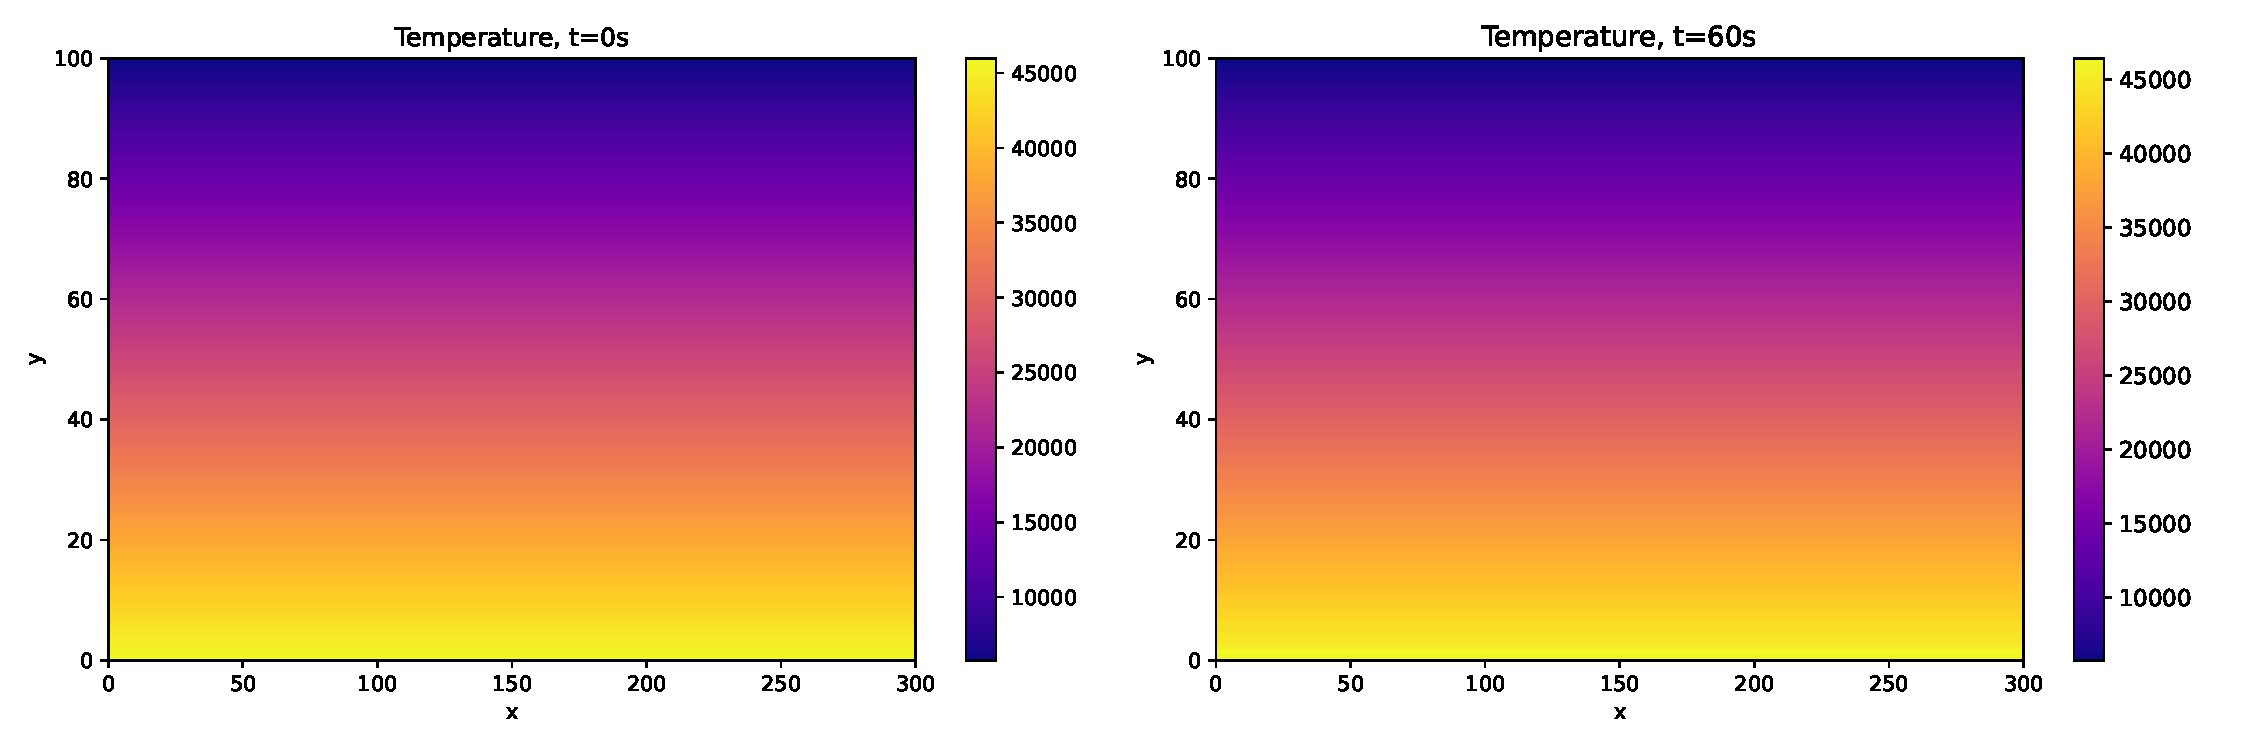
\includegraphics[width = 0.47\textwidth]{figures/sanity_check.pdf} 
    \caption{The initial temperature distribution in the xy-space for a system initialized with no initial temperature perturbations, only affected by the gravitation in the y-direction (left), and the temperature distribution in the same space after being evolved in time 60s (right)}
    \label{fig:sanity}
\end{figure}

\subsection{Behavioural Analysis}
\subsubsection{A Single Gaussian Temperature Distribution}
The model is tested further by implementing a single Gaussian perturbation in the initial temperature distribution, and checking the initialization by visualizing the temperature and density distributions in the Figure \ref{fig:single_both}.
\begin{figure}[H]
    \centering
    \includegraphics[width =0.47\textwidth]{figures/initial_two_single.pdf} 
    \caption{The initial temperature (left) and density (right) distributions in the system initialized with a single temperature perturbation defined by the variables $A=60000 K, x_0=6\times 10^6, y_0=0, \sigma_x=5\times 10^5, \sigma_y=3\times 10^6$}
    \label{fig:single_both}
\end{figure}
\begin{figure*}
    \centering
    \includegraphics[width=1\textwidth]{figures/single_collage.png} 
    \caption{The distribution of temperatures (indicated by color maps) and direction of movement (indicated by vector fields) in the xy-space, for a system initialized with a single temperature perturbation defined by the variables $A=60000 K, x_0=6\times 10^6, y_0=0, \sigma_x=5\times 10^5, \sigma_y=3\times 10^6$. Snapshots taken at times t=0:35, t=2:01, t=3:34, t=5:33, with links to animation over the entire time-interval of 600 seconds in the Appendix A, Section \ref{sec:appendix_A}}
    \label{fig:single_shots}
\end{figure*}
\begin{figure*}
    \centering
    \includegraphics[width=1\textwidth]{figures/single_velocity_collage.png} 
    \caption{The velocity of the gas indicated by color maps and direction of movement indicated by vector fields in the xy-space, for a system initialized with a single temperature perturbation defined by the variables $A=60000 K, x_0=6\times 10^6, y_0=0, \sigma_x=5\times 10^5, \sigma_y=3\times 10^6$. Snapshots taken at times t=0:35, t=2:01, t=3:34, t=5:33, with links to animation over the entire time-interval of 600 seconds in the Appendix A, Section \ref{sec:appendix_A}}
    \label{fig:single_vel}
\end{figure*}
\begin{figure*}
    \centering
    \includegraphics[width=1\textwidth]{figures/single_densities_collage.png} 
    \caption{The distribution of mass density in the xy-space, and direction of movement for a system initialized with a single temperature perturbation defined by the variables $A=60000 K, x_0=6\times 10^6, y_0=0, \sigma_x=5\times 10^5, \sigma_y=3\times 10^6$. Snapshots taken at times t=0:35, t=2:01, t=3:34, t=5:33, with links to animation over the entire time-interval of 600 seconds in the Appendix A, Section \ref{sec:appendix_A}}
    \label{fig:single_dens}
\end{figure*}
The behaviour of rising gasses in the xy-space is subsequently simulated by evolving the system in time. Snapshots are taken of the distribution of temperatures in the xy-space at different times t=0:35, t=2:01, t=3:34, t=5:33, visualized in the Figure \ref{fig:single_shots}. Also the direction of movement is denoted by vector fields in each snapshot. The velocity distribution in the space is visualized Figure \ref{fig:single_vel}, and the mass density in Figure \ref{fig:single_dens}, by snapshots taken at the same times. \\ 

A detailed analysis on how the average of the following variables are detailed in the correlated figures; average internal energy and momentum density in Figure \ref{fig:e_rhov}, average energy flux and temperature in Figure \ref{fig:en_t} and average mass density and speed in Figure \ref{fig:rho_v}.
\begin{figure}[H]
    \centering
    \includegraphics[width = 0.47\textwidth]{figures/single_collage1.png} 
    \caption{The average internal energy (left) and momentum density (right) in the system as a function of time. System initialized with a single temperature perturbation defined by the variables $A=60000 K, x_0=6\times 10^6, y_0=0, \sigma_x=5\times 10^5, \sigma_y=3\times 10^6$}
    \label{fig:e_rhov}
\end{figure}
\begin{figure}[H]
    \centering
    \includegraphics[width = 0.47\textwidth]{figures/single_collage2.png} 
    \caption{The average energy flux (left) and temperature (right) in the system as a function of time. System initialized with a single temperature perturbation defined by the variables $A=60000 K, x_0=6\times 10^6, y_0=0, \sigma_x=5\times 10^5, \sigma_y=3\times 10^6$}
    \label{fig:en_t}
\end{figure}
\begin{figure}[H]
    \centering
    \includegraphics[width = 0.47\textwidth]{figures/single_collage3.png}
    \caption{The average mass density (left) and speed (right) in the system as a function of time. System initialized with a single temperature perturbation defined by the variables $A=60000 K, x_0=6\times 10^6, y_0=0, \sigma_x=5\times 10^5, \sigma_y=3\times 10^6$}
    \label{fig:rho_v}
\end{figure}
The evolution of energy flux in the system is visualized in the Figure \ref{fig:single_enflux}, by snapshots of the behaviour as a function of the vertical distance at the times t=0:35, t=3:34, t=5:00, t=8:32. \\
\begin{figure*}
    \centering
    \includegraphics[width =1\textwidth]{figures/single_energy_flux.png}
    \caption{The evolution of energy flux for a system initialized with a single temperature perturbation defined by the variables $A=60000 K, x_0=6\times 10^6, y_0=0, \sigma_x=5\times 10^5, \sigma_y=3\times 10^6$. Snapshots taken at times t=0:35, t=3:34, t=5:00, t=8:32 with links to animation over the entire time-interval of 600 seconds in the Appendix A, Section \ref{sec:appendix_A} }
    \label{fig:single_enflux}
\end{figure*}

A cooler perturbation is initialized and visualized in Figure \ref{fig:small_single} in order to make sure that the method does not affect the implementation of the naturally occurring hydrostatic equilibrium.
\begin{figure}[H]
    \centering
    \includegraphics[width = 0.47\textwidth]{figures/initial_two_single_small.pdf}
    \caption{Initial temperature (left) and mass density (right) distributions, for a system initialized with a single temperature perturbation $A=8000 K, x_0=5\times 10^5, y_0=0, \sigma_x=3\times 10^5, \sigma_y=3\times 10^6$}
    \label{fig:small_single}
\end{figure}
\begin{figure*}
    \centering
    \includegraphics[width =1\textwidth]{figures/five_collage.png} 
    \caption{The temperature distribution (denoted by color maps) and direction of movement (indicated by vector fields) in the xy-space, for a system initialized with a five distinct temperature perturbations defined by the variables presented in Table \ref{tab:six}. Snapshots taken at times t=0:35, t=1:01, t=2:01, t=3:34, t=5:00, t=8:05, with links to animation over the entire time-interval of 600 seconds in the Appendix A, Section \ref{sec:appendix_A}}
    \label{fig:five_shots}
\end{figure*}





\subsubsection{Multiple Gaussian Temperature Distributions}
The model is consequently utilized to simulate the behaviours of a system initialized with five distinct Gaussian perturbations in the initial temperature, defined by the variables presented in Table \ref{tab:six}. 
The initial distribution of the temperature and mass density for the system defined by these variables is visualized in Figure \ref{fig:five_initial}. \\
\begin{figure}[H]
    \centering
    \includegraphics[width =0.47\textwidth]{figures/initial_two_five.pdf} 
    \caption{Initial temperature and mass density distribution for system initialized with perturbations defined by variables presented in Table \ref{tab:six}.}
    \label{fig:five_initial}
\end{figure}

The behaviour of rising parcels in the xy-space as time passes is modelled and visualized by the snapshots taken for temperature at the times t=0:35, t=1:01, t=2:01, t=3:34, t=5:00 and t=8:05, presented in the Figure \ref{fig:five_shots}.% \newpage
\begin{table}[H]
\caption{Variables used to define five distinct perturbations in the xy-space.}
    \begin{tabular*}{0.47\textwidth}{@{\extracolsep{\fill}}ccccc}
    \toprule
    \textbf{Amplitude [K]:} &  \textbf{$x_0$ [m]:}  & \textbf{$y_0$ [m]:} &  \textbf{$\sigma_x$ [m]:} &  \textbf{$\sigma_y$ [m]:}  \\
    \hline
    $6\cdot 10^4$  &  $2\cdot 10^6$    & $0$ & $5\cdot 10^5$ &$3\cdot 10^6$ \\
    $4\cdot 10^4$  &  $4\cdot 10^6$    & $0$ & $5\cdot 10^5$ &$3\cdot 10^6$ \\
    $6\cdot 10^4$  &  $6\cdot 10^6$  & $0$ & $5\cdot 10^5$ &$3\cdot 10^6$ \\
    $4\cdot 10^4$  &  $8\cdot 10^6$    & $0$ & $5\cdot 10^5$ &$3\cdot 10^6$ \\
    $6\cdot 10^4$  &  $10\cdot 10^6$   & $0$ & $5\cdot 10^5$ &$3\cdot 10^6$ \\
    \end{tabular*}
    \label{tab:six}
\end{table}




\section{Discussion}
From the Figure \ref{fig:sanity} one can read a successful initialization of the hydrostatic equilibrium within the 2D space constructed. The plot showing comparing the condition at t=0 and the condition after 60 seconds has passed, confirms the temperature distribution to remain constants. The equilibrium is upheld, as expected, as there are no disruptions. \\

The Figure \ref{fig:single_both} confirms the implementation of the Gaussian temperature distribution within the system. The Figure \ref{fig:small_single} confirms that the total initial temperature distribution is a sum of the natural temperature distribution denoting the hydrostatic equilibrium, and the disturbance created by the method recently introduced. \\

The Figure \ref{fig:single_shots} shows the rising gas colliding with the top vertical boundary of the volume-space, and it's spread thereafter. From these snapshots one can read a successful implementation of the boundaries of the system. The vector field visualizes the rapidness and direction of the change in the movement of the gas when it collides with either the borders of the space, or itself. From the evolution of this vector field, and the prominent pattern emerging as time passes, it is clear that two vortex have appeared as a result of these collisions occurring. Figure \ref{fig:single_vel} and Figure \ref{fig:single_dens} visualizes the distribution of mass density and velocity in the same space, from which we can gather a clearer picture of the motion of the heated gas. The mass density remains evenly distributed through the space, but does nevertheless follow the movement of the heated gas slightly, before it gathers at the bottom of the 2D space following the collision with the upper boundary. This is to be expected, as result of the gravitational pull working on the gas in negative y-direction. The color maps indicating velocity forms clear patterns, denoting streams forming as a result of collision with other heated gas streams, and the boundaries applied to the space. Thee function of these plots is to emphasize the vector field applied to all three figures, and subsequently provide a clearer image of the movement of gas occurring in the simulation.    \\

The Figure \ref{fig:e_rhov} shows us a linear increase in average momentum density as time passes. The average internal energy displays a very different behaviour, where the curve increases abruptly in the interval between 0 and 300 seconds, but stabilizes around 0.04 $[J/m^3]$ thereafter. This is simply explained by the direction of travel of the majority of the gas - at around 300 seconds, the heated stream has collided with the vertical boundary, and the energy becomes more evenly distributed in the space. \\
\newpage
The Figure \ref{fig:en_t} visualizes the linear increase in values of the average energy flux, from a value of -1 $[W/m^2]$ at t=0 to 0.5 $[W/m^2]$ at t=500s, where there is a dip in the function. The negative energy flux values is simply explained by the average direction of movement of the gas being negative in the interval in question. The behaviour of the average temperature visualized in the same figure shows an increase of positive values until it peaks at about 400 seconds, before the function dips again, until the duration of the simulation approaches 500 seconds. In the interval 500-600 seconds, the temperature stabilizes at around 0.8[K]. This is explained by the temperature visualized being relative to the initial value, and as time passes, the temperature becomes more evenly distributed in the space, as observed in the temperature distributions for a single temperature perturbation visualized in Figure \ref{fig:single_shots} and five perturbations in Figure \ref{fig:five_shots}. \\

The Figure \ref{fig:rho_v} displays an average mass density that remains relative stable at 0 until the simulation has ran for 300 seconds. In the interval 300-600 seconds, the graph decreases dramatically into the negatives. The average speed visualized in the same figure increases linearly in the time interval 0-450 seconds where it peaks and decreases in the interval 450-600 seconds. This indicates a decrease in the speed of the gas flowing downward on average. In the interval 0-300 seconds, the average speed is also displayed as negative - a result of the gas moving strictly toward the top of the y-dimension in this interval. \\

The Figure \ref{fig:single_enflux} shows how the average energy flux as a function of the y-coordinate behaves as time passes. From these snapshots, one can see an energy flux that is rather unstable when y is small, but becomes more stable as the distance increases. Furthermore, an it is clear that the graph is displaying an oscillating motion, which can be accentuated when looking at the GIF \ref{gif:single_energy} for the entire time interval. The displacement of the graph indicating the vertical energy flux, has the physical interpretation of heated gas travelling at a distance y. It is clear that the oscillation hits the y-boundary, where it subsequently moves toward lower y-values, and oscillates in the scaled vertical distance interval 0-0.5 for the remainder of the simulation. This has to do with the more even temperature distribution - energy becomes more evenly distributed in the space, as it is conserved. This, we know is a direct consequence of the definition we chose of energy, momentum and continuity equations - source and sink terms, as well as stress tensors, have been excluded.  \\

After confirming the sanity of the model, we initialize a system defined by five different temperature perturbations, and present the initial temperature and mass density distributions in Figure \ref{fig:five_initial}. The plots show a successful implementation of the multiple disruptions into the system. Snapshots of the observed behaviours of temperature and velocity in the xy-volume as time passes is presented in the Figure \ref{fig:five_shots}. These five different temperature deviations are centered symmetrically around the midpoint on the x-axis, with amplitudes similarly symmetric, which we can see results in symmetric temperature and velocity distributions as time passes. As the different temperature-streams interact with each other and the borders of the system, it is clear from the vector fields that vortexes arises in the space as a result of the changing movement directions. This is exactly as one would expect for such a system, where mass and momentum is expected to be conserved. \\

\newpage
\section{Conclusion}
The model seems to be successfully simulating the behaviours occurring for rising parcels of gas in the conservative zones in a star. \\

We've developed a model which seems to be realistic, and used it to visualize the properties of fluid mechanics. By implementing a method that initializes perpetuation in the initial temperature, we manage to simulate the spread of temperature and energy in the xy-space, imitating the heated gas raising in the continuous convective-zone at the surface of the star. From our plots, it is clear that the spread of the gas is hindered by the gravitational pull and friction from the flow of gas it collides with, which results in a mushroom-like pattern.



\section{Reflection}
This project has taught me a lot about fluid mechanics in general. I initially had a lot of problems getting ffmpeg to work and creating the mp4 videos, which is an issue I eventually solved by making direct changes to the FVis3 file. This is something I initially did want to avoid, but as I got frustrated I decided to do it anyway, so that the animations could at least be visualised and added to my report. Furthermore, I had some issues defining the discretized variables as well, but via trial and error in coding, I arrived at both an adequate analysis of theory and a working model. 


\section{Appendix A : Links to Animations}\label{sec:appendix_A}
\subsection{Single Temperature Perturbation}
\href{https://imgur.com/viXac8d}{Temperature}\label{gif:single_temperature} (https://imgur.com/viXac8d)\\
\href{https://imgur.com/kEzD4Cq}{Velocity}\label{gif:single_velocity} (https://imgur.com/kEzD4Cq)\\
\href{https://imgur.com/OYZ9TlO}{Density}\label{gif:single_density} (https://imgur.com/OYZ9TlO)\\
\href{https://imgur.com/RQZ687J}{Energy Flux}\label{gif:single_energy} (https://imgur.com/RQZ687J)\\
\subsection{Five Temperature Perturbations}
\href{https://imgur.com/GKBQTHT}{Temperature}\label{gif:five_temperature} (https://imgur.com/GKBQTHT)\\
\href{https://imgur.com/sNONzEW}{Energy Flux}\label{gif:five_energy} (https://imgur.com/sNONzEW)\\

%https://imgur.com/a/la6awK8

\bibliographystyle{plain}
\bibliography{references}
\end{document}